\section{zombie.c}

	Muestre la pantalla de ejecución del programa y ejecute de manera adicional en una terminal diferente el comando ps -ae.

	\begin{center}
		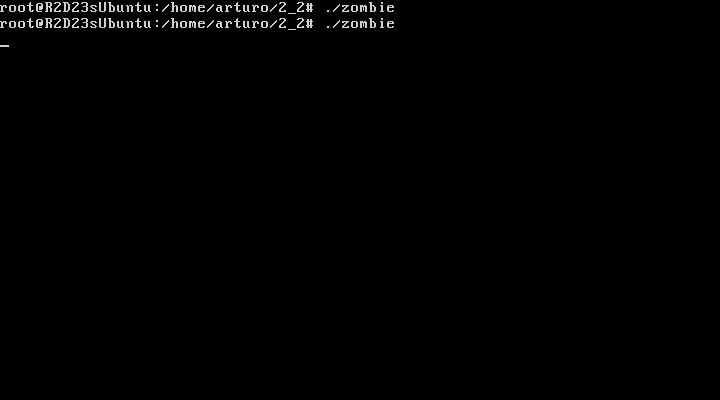
\includegraphics[width=\linewidth]{imagenes/zombie.png}
		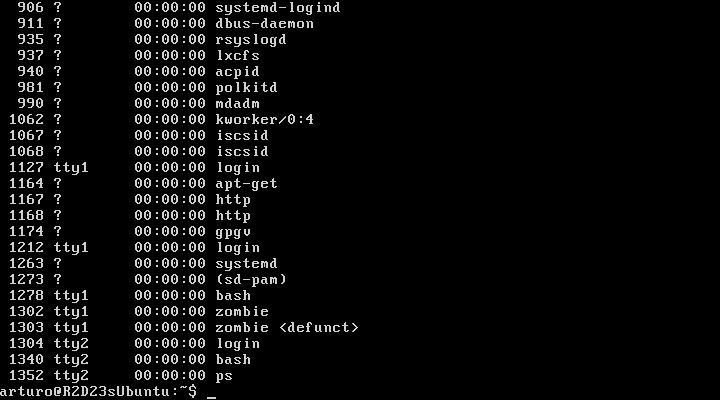
\includegraphics[width=\linewidth]{imagenes/zombie_ps.png}
	\end{center}

	Realice lo siguiente

	\begin{itemize}

		\item Investigue en la bibliografía proporcionada para la asignatura, el diagrama de estados de procesos en LINUX y describa de manera cuáles son las condiciones que hacen que se pase a cada estado
		
	\begin{tcolorbox}
	
	Estos son los estados de los procesos de Linux\cite{o'reilly}:
	\begin{itemize}
	\item \textbf{TASK\_RUNNING}\\
	El proceso ya está siendo ejecutado o está en espera de ser ejecutado.
	\item \textbf{TASK\_INTERRUPTIBLE}\\
	Proceso suspendido que puede reanudar a TASK\_RUNNING dada una señal.
	\item \textbf{TASK\_UNINTERRUPTIBLE}\\
	Proceso suspendido que no puede reanudar normalmente a TASK\_RUNNING dada una señal.
	\item \textbf{TASK\_STOPPED}\\
	Estado que indica que un proceso ha acabado.
	\item \textbf{TASK\_ZOMBIE}\\
	Estado que indica que un proceso ha acabado, pero no puede ser removido apropiadamente pues el padre no puede ser reportado de datos del proceso que podría necesitar. (Según la bibliografía, esto sucede cuando el proceso padre no sale de \textit{wait()})
	\end{itemize}
	\end{tcolorbox}

	\item Tomando como referenca el diagrama obtenido en el punto anterior, explique de manera detallada los estados por los que pasa el proceso padre y el proceso hijo durante la ejecución del programa
		
	\begin{tcolorbox}
	
	\begin{itemize}
	\item El proceso padre empieza en estado TASK\_RUNNING.
	\item El proceso padre llama la función \textit{fork()} y obtiene un hijo de mismo código.
	\item Ambos procesos en estado TASK\_RUNNING entran al switch case.
	\item El padre pasa a TASK\_UNINTERRUPTIBLE con \textit{sleep()}.
	\item El proceso hijo termina, pero pasa a TASK\_ZOMBIE, pues su padre sigue en TASK\_UNINTERRUPTIBLE.
	\item Ambos procesos pasan a TASK\_STOPPED 
	\end{itemize}
	
	\end{tcolorbox}
	
	\end{itemize}

	\begin{itemize}

		\item perror
	\begin{tcolorbox}
		Esta función produce un mensaje que describe al último error obtenido durante una llamada al sistema o una función de biblioteca.
	\end{tcolorbox}
		\item fork
	\begin{tcolorbox}
		Crea un proceso hijo duplicando el proceso padre.
	\end{tcolorbox}

	\end{itemize}

